\documentclass[a4paper,10pt]{article}
\usepackage[utf8]{inputenc}
\usepackage{amssymb}
\usepackage[german]{babel}
\usepackage{graphicx}
%\usepackage{cite}
\usepackage{bibgerm}

%opening
\title{}
\author{Margrit Dittmann}

\begin{document}

\maketitle
\tableofcontents
\pagebreak

%\begin{abstract}

%\end{abstract}

%Die M\"oglichkeiten der theoretischen Informatik werden meiner Meinung nach oft nicht richtig wahrgenommen. Die Lehre der Automatentheorie geh\"ort zu den Grundlagenveranstaltungen im Informatikstudium. Wie ich in meiner Zeit als Tutorin feststellen musste, haben immer wieder viele Studierende Probleme mit der mathematischen Darstellung und den Beweisenverfahren. Die angestrebte Formalisierung soll den Studierenden die M\"oglichkeit bieten, die Theorie aus einem anderen Blickwinkel zu betrachten.

\section{Was ist das Ziel der Arbeit?}

Das Ziel dieser Arbeit ist die Darstellung eines Teilgebietes der Automatentheorie und einigen dazugeh\"origen Verfahren mit Hilfe von den Sytemen NuPRL, Coq oder Idris. Es werden nur deterministische und nicht-deterministische endliche Automaten betrachtet. Die zu ber\"ucksichtigen Verfahren sind:

\begin{itemize}
 \item DEA/NEA
 \item regul\"are Ausdr\"ucke
 \item regul\"aren Ausdr\"ucken $\Leftrightarrow$ endliche Automaten
 \item deterministische Automaten $\Leftrightarrow$ nicht-deterministische Automaten
 \item Pumping Lemma f\"ur regul\"are Sprachen
 \item Satz von Myhill-Nerode
\end{itemize}

Wichtige Aspekte bei der Modellierung sind Lesbarkeit und Erweiterbarkeit auf andere Automatenmodelle. Eine M\"oglichkeit w\"are eine vergleichende Betrachtungsweise zwischen den einzelnen Systemen und deren Formalisierungen von Automaten. Hierbei ist die Anzahl der umsetzbaren Verfahren eher begrenzt. Die andere, wahrscheinliche Vorgehensweise w\"are sich eines der Systeme auszuw\"ahlen um so viele Verfahren wie m\"oglich umzusetzen.

\section{Wie sollen das Ziel erreicht werden?}
Zur Erreichung des Ziels muss ein Formalismus zur Darstellung der Automaten und der Verfahren entwickelt werden. 
\begin{itemize}
 \item Analyse der Ans\"atze f\"ur Coq und NuPRL
 \item Modellierung der Automaten im jeweiligen System
 \item Modellierung regul\"arer Ausdr\"ucke
 \item Formalismen entwickeln zur Umsetzung der Verfahren
 \begin{itemize}
  \item regul\"aren Ausdr\"ucken $\Leftrightarrow$ endliche Automaten
  \item deterministische Automaten $\Leftrightarrow$ nicht-deterministische Automaten
  \item Pumping Lemma f\"ur regul\"are Sprachen
  \item Satz von Myhill-Nerode
 \end{itemize}
\end{itemize}
Um sp\"atere Grundlegende Probleme zu vermeiden, sollten schon bei der Darstellung der Automaten die umzusetzenden Verfahren ber\"ucksichtigt werden.

\section{Zeitliche Ablaufplanung}
Die effektive Arbeitszeit betr\"agt ca. 24h pro Woche. Für die beiden Varianten ist eine unterschiedliche Zeitplanung zu ber\"ucksichtigen. Die Entscheidung, ob es eine vergleichende Arbeit wird, oder die Verfahren nur in einem System beschrieben werden, soll Anfang KW 11 fallen. In diesem Zeitraum werden gleichzeitig die Grundlagen der Automatentheorie, der Verfahren, der regul\"aren Sprachen wiederholt und die wichtigen Punkte herausgearbeitet. Dies sollte nicht mehr als 2 Tage in Anspruch nehmen.
\begin{enumerate}
 \item zur Vorbereitung, Einarbeitung in:
 \begin{itemize}
  \item Coq bereits teilweise geschehen
  \item NuPRL (KW 7+8)
  \item Idris (KW 9+10)
 \end{itemize}
 \item Variante 1: vergleichende Arbeit
 \begin{itemize}
  \item Automaten (DEA/NEA) in den Systemen implementieren (KW 11-18)
  \item regul\"are Ausdr\"ucke (KW 19+20)
  \item regul\"are Ausdr\"ucken $\Leftrightarrow$ endliche Automaten (KW 21-23)
  \item deterministische Automaten $\Leftrightarrow$ nicht-deterministische Automaten (KW 23-25)
  \item Die weiteren Punkte werden Aufgrund der Komplexit\"at nicht ber\"ucksichtigt.
 \end{itemize}
 \item Variante 2: beschreibende Arbeit
 \begin{itemize}
  \item Implementierung der Automaten (KW 11-14)
  \item Umsetzung und Test aller unter 1. beschrieben Punkte (ca 2 Wochen pro Punkt), wobei die Automatenmodellierung wahrscheinlich angepasst werden muss. Der Schwerpunkt liegt auf der lesbaren Implementierung des Pumping Lemmas f\"ur regul\"are Sprachen.
 \end{itemize}
 \item Fertigstellung
 \begin{itemize}
  \item Fertigstellung der jeweiligen Implementierung (KW 25)
  \item schriftliche Ausarbeitung \"uber den ganzen Zeitraum und \"Uberarbeitung (KW 26-30)
  \item Endkontrolle und Druck (KW 30+31)
 \end{itemize}
\end{enumerate}


%Hier steht irgendwann mal ne Einleitung

\section{Entscheidung}
Die zur Auswahl stehenden Systeme sind NuPRL, Coq und Idris, wobei es sich bei Coq und NuPRL um interaktive Beweissysteme auf Basis vom ML handelt. Idris ist an die Haskell Syntax angelehnt ist. In allen drei Systemen stehen Taktiken zur Beweisf\"uhrung und zur Verbesserung der Lesbarkeit zur Verf\"ugung und es handelt sich um funktionale Programmiersprachen h\"oheren Levels. %Formulierung 

In den Systemen NuPRL und Coq gibt es bereits erste Realisierungen von Automaten. Die NuPRL Realisierung ist aus dem Jahr 1986 \cite{Krei86} und k\"onnte als Ideengeber angesehen werden, da sich das System mit der Zeit stark ver\"andert hat.  %Formulierung

Die NuPRL Architektur besteht aus einer Wissensbasis als Zentrum, die durch die Nutzer stetig erweitert werden kann, und anliegenden Schnittstellen, wie beispielsweise der Benutzeroberfl\"ache. Sie bietet ebenfalls automatische Tools wie Entscheidungsprozeduren, Theorembeweiser, Beweisplaner, Modelchecker, Rewrite Enginges an. %Formulierung

\begin{figure}[h!] %  figure placement: here, top, bottom, or page
   \centering
   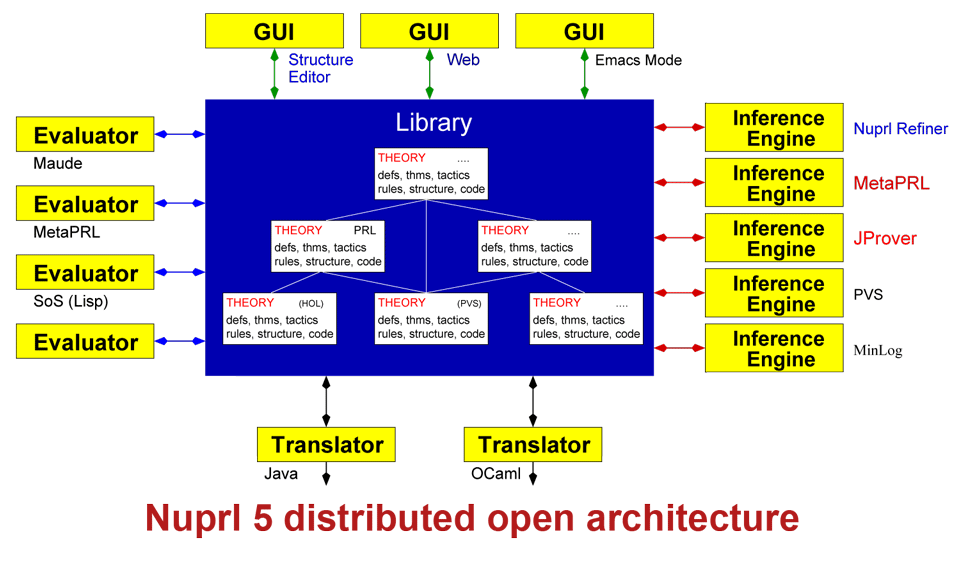
\includegraphics[width=1.0\textwidth]{NuPRL-Architiktur.PNG} 
   \caption{NuPRL 5 Architektur \cite{Nu5arch}}
   \label{fig:example}
\end{figure}

Verschiedene Nutzer k\"onnen parallel auf die Wissensbasis zugreifen und alle \"Anderungen werden umgehend \"ubertragen, so dass im Falle eines Systemausfalls beim Benutzer, keine Daten verloren gehen. Bei \"Anderungen an Objekten werden diese nicht \"uberschrieben sondern es wird eine neue Version vom jeweiligen Objekt erstellt. Dieses Vorgehen erm\"oglicht es, \"altere Versionen wieder herzustellen um somit beispielsweise mehrere Beweise eines Theorems zu erstellen. 

Die Komplexit\"at des Systems mit den vielen Schnittstellen und den verschiedenen graphischen Darstellungsm\"oglichkeiten f\"ur den Benutzer erscheint am Anfang sehr un\"ubersichtlich und der Code ist nicht unbedingt intuitiv lesbar. %zu komplex f�r Einsteiger

%- \begin{quotation}
%   The Nuprl LPE (logical programming environment) is an open , distributed architecture that integrates all its key subsystems as independent components and, by using a flexible knowledge base as its central component, supports the interoperability of current proof technology.
%  \end{quotation}

Die Realisierungen von endlichen Automaten in Coq sind deutlich j\"unger. So wird ein Formalismus zur Darstellung von regul\"aren Ausdr\"ucken im Jahr 2011 beschrieben \cite{RA2011}. Es gibt eine ganze Reihe von Ans\"atzen, die in dieser Arbeit betrachtet und bez\"uglich ihrer Verwendbarkeit analysiert werden.

Coq ist ein intuitionistischer Theorembeweiser mit einer einfach strukturierten Benutzeroberfl\"ache, der CoqIDE. Es gibt diverse Online Tutorials zur Installation und Anwendung \cite{TuCoq}. Die dem System zugrundeliegende Theorie ist der \glqq Calculus of Inductive Constructions\grqq{} \cite[S. V]{CoqBuch}. Weiterhin werden Exporte in g\"anginge Formate, wie XML, HTML und \LaTeX angeboten \cite{Export}. Die aktive Gemeinschaft u.a. in Form einer Mailing Liste, reagiert schnell auf Fragen und ist leicht zug\"anglich \cite{Mail}.
 
Idris bietet ebenfalls ein funktionales Interface, welches die Interaktion mit einer externen C Bibliothek erm\"oglicht. Die Verwendung der Taktik basierten Beweisf\"uhrung wurde von Coq beeinflusst \cite{IdCoq}. Eine aktive Gemeinschaft ist ebenfalls u.a. in Form einer Mailing Liste gegeben \cite{MailIdris}. Exporte sind u.a. in Javascript m\"oglich \cite{IdrisTutorial}. Allerdings bietet Idris von sich aus keine Benutzeroberfl\"ache und kann entweder \"uber Vim oder Emacs benutzt werden \cite{IdrisIDE}. Weiterhin muss man beim Programmieren beachten, dass gewisse Argumente exakt untereinander stehen, da es sonst zu Problemen f\"uhren kann \cite{IdrisTutorial}.
%gibt es die ? Variante, wenn ein Beweis noch nicht komplett gef�hrt wurde auch in Coq?
 
Ein weiterer wichtiger Aspekt f\"ur die sp\"atere Anwendung ist eine einfache Installation des zugrundeliegenden Systems unabh\"agig vom Betriebssystem. Dies ist sowohl bei Coq, als auch bei Idris gegeben. NuRPL l\"auft nur \"uber eine virtuelle Maschine und Installationsinformationen sind nur sehr schwer zu finden.

Coq und Idris sind zwei Systeme, die im Moment von zwei aktiven Communities gepflegt und weiterentwickelt werden. Die aktuelle Coq Version 8.4pl5 wurde am 31.10.2014 ver\"offentlicht \cite{Coq84} und die 8.5 beta 1 Version kam am 21.01.2015 \cite{Coq85}. Bei Idris erschien das letzte Release 0.9.16 am 15. Januar 2015 \cite{IdRel}. Im Gegensatz dazu ist bei NuPRL das letzte Release, NuPRL 5, 2000 erschienen \cite{Nu5}. Aus diesem Grund und wegen der Probleme bei dem Beziehen der Plattform und der Installationsprobleme klammere ich NuPRL aus meinen weiteren Betrachtungen aus.


%\input{DEA_NEA.tex}
%\input{regSprachen_DEA.tex}
%\input{Aequivalenz.tex}
%\input{Myhill_Nerode.tex}
%\input{Pumping_Lemma.tex}
%\input{Didaktik_Anwendungsmoeglichkeiten}
%\input{Zusammenfassung.tex}

\newpage
\addcontentsline{toc}{section}{Literatur}
\bibliography{Literatur.bib}
\bibliographystyle{geralpha}
%Zitate dann mit \cite{} machen
\listoffigures
\listoftables
\end{document}
